\documentclass[10pt,a4paper,spanish]{report}

\usepackage[light,condensed,math]{iwona}
\usepackage[T1]{fontenc}

\usepackage[spanish]{babel}
\usepackage[utf8]{inputenc}
\usepackage{amsmath, amsthm}
\usepackage{amsfonts, amssymb, latexsym}
\usepackage{enumerate}
\usepackage[official]{eurosym}
\usepackage{graphicx}
\usepackage{graphics}
\usepackage[usenames, dvipsnames]{color}
\usepackage{colortbl}
\usepackage{multicol}
\usepackage{multirow}
\usepackage{fancyhdr}
\usepackage{fancybox}
\usepackage{pseudocode}
\usepackage[all]{xy}
\usepackage{minted}
\usepackage{tikz}
\usepackage{pgfplots}
\usepackage{subfigure}
\usepackage{epigraph}



% \pgfplotsset{compat=1.5}

% a4large.sty -- fill an A4 (210mm x 297mm) page
% Note: 1 inch = 25.4 mm = 72.27 pt
%       1 pt = 3.5 mm (approx)
\topmargin      0 mm    % top margin less 1 inch
\headheight     0 mm    % height of box containing the head
\headsep        10 mm    % space between the head and the body of the page
\textheight     250 mm
\footskip       14 mm    % distance from bottom of body to bottom of foot

% % horizontal page layout -- one inch margin each side
% \oddsidemargin    0   mm    % inner margin less one inch on odd pages
% \evensidemargin   0   mm    % inner margin less one inch on even pages
% \textwidth      159.2 mm    % normal width of text on page


\usepackage[bookmarks=true,
            bookmarksnumbered=false, % true means bookmarks in
                                     % left window are numbered
            bookmarksopen=false,     % true means only level 1
                                     % are displayed.
            colorlinks=true,
            linkcolor=webblue]{hyperref}
\definecolor{webgreen}{rgb}{0, 0.5, 0} % less intense green
\definecolor{webblue}{rgb}{0, 0, 0.5}  % less intense blue
\definecolor{webred}{rgb}{0.5, 0, 0}   % less intense red

\newcommand{\HRule}{\rule{\linewidth}{0.5mm}} % regla horizontal para  el titulo

\pagestyle{fancy}
%con esto nos aseguramos de que las cabeceras de capítulo y de sección vayan en minúsculas

\renewcommand{\sectionmark}[1]{%
      \markright{\thesection\ #1}}
\fancyhf{} %borra cabecera y pie actuales
\fancyhead[LE,RO]{\textcolor[rgb]{0.5,0.8,0.9}{\bfseries\thepage}}
\fancyhead[LO]{\bfseries Braulio Vargas}
\renewcommand{\headrulewidth}{0.5pt}
\renewcommand{\footrulewidth}{0pt}
\addtolength{\headheight}{0.5pt} %espacio para la raya
\fancypagestyle{plain}{%
      \fancyhead{} %elimina cabeceras en páginas "plain"
      \renewcommand{\headrulewidth}{0pt} %así como la raya
}

 \newmintedfile[mycpp]{c++}{
    linenos,
    numbersep=5pt,
    gobble=0,
    frame=lines,
    framesep=2mm,
}

\newmintedfile[mypython]{python}{
    linenos,
    numbersep=5pt,
    gobble=0,
    frame=lines,
    framesep=2mm,
}

%%%%% Para cambiar el tipo de letra en el título de la sección %%%%%%%%%%%
\usepackage{sectsty}
\chapterfont{\fontfamily{pag}\selectfont} %% for chapter if you want
\sectionfont{\fontfamily{pag}\selectfont}
\subsectionfont{\fontfamily{pag}\selectfont}
\subsubsectionfont{\fontfamily{pag}\selectfont}

% Indentacion fuera
\setlength{\parindent}{0pt}
\setlength{\parskip}{1ex plus 0.5ex minus 0.2ex}

\usepackage{titlesec}

\titleformat{\chapter}{\normalfont\huge\center}{--- \thechapter ---}{20pt}{}

\titleformat
{\chapter} % command
[display] % shape
{\Huge\center\bfseries} % format
{--- \thechapter ---} % label
{0.5ex} % sep
{
    \rule{\textwidth}{1pt}
    \vspace{1ex}
    \centering
} % before-code
[
\vspace{-0.5ex}%
\rule{\textwidth}{0.3pt}
] % after-code


%%%%%%%%%%%%%%%%%%%%%%%%%%%%%%%%%%%%%%%%%%%%%%%%%%%%%%%%%%%%%%%%%%%%%%%%%%%%%%%%%%%%%%%%%%
%                 APENDICES
%%%%%%%%%%%%%%%%%%%%%%%%%%%%%%%%%%%%%%%%%%%%%%%%%%%%%%%%%%%%%%%%%%%%%%%%%%%%%%%%%%%%%%%%%%
\usepackage{appendix}
\renewcommand{\appendixname}{\fontfamily{pag}Apéndice}
\renewcommand{\appendixtocname}{\fontfamily{pag}\textcolor[rgb]{0.1,0.2,1}Apéndice:\\\textcolor[rgb]{0.1,0.2,1}Ejemplos y \textcolor[rgb]{0.1,0.2,1}Ejercicios \textcolor[rgb]{0.1,0.2,1}Resueltos}
\renewcommand{\appendixpagename}{\fontfamily{pag}\textcolor[rgb]{0.1,0.2,1}Apéndice:\\\textcolor[rgb]{0.1,0.2,1}Ejemplos y \textcolor[rgb]{0.1,0.2,1}Ejercicios \textcolor[rgb]{0.1,0.2,1}Resueltos}
\usepackage{cancel}
\usepackage{geometry}
\usepackage{xcolor}
% \usepackage{graphicx}

\definecolor{titlepagecolor}{rgb}{0.0, 0.28, 0.67}
\definecolor{namecolor}{rgb}{0.55, 0.57, 0.67}

%%%%%%%%%%%%%%%%%%%%%%%%%%%%%%%%%%%%%%%%%%%%%%%%%%%%%%%%%%%%%%%%%%%%%%%%%%%%%%%%%%%%%%%%%%%%%%%%%%%%%%%%%%%%%%%%%%%%%%%%%%%%%%%%%%%%%%%%%%%%%%%%%%%%



%%%%%%%%%%%%%%%%%%%%%%%%%%%%%%%%%%%%%%%%%%%%%%%%%%%%%%%%%%%%%%%%%%%%%%%%%%%%%%%%%%%%%%%%%%%%%%%%%%%%%%%%%%%%%%%%%%%%%%%%%%%%%%%%%%%%%%%%%%%%%%%%%%%%

\begin{document}
\begin{titlepage}
\newgeometry{left=7.5cm} %defines the geometry for the titlepage
\pagecolor{titlepagecolor}
\noindent
% \includegraphics[width=2cm]{logo.jpg}\\[-1em]
\color{white}
\makebox[0pt][l]{\rule{1.3\textwidth}{3pt}}
\par
\noindent
\Large{\textbf{\textsf{Guión de Prácticas}} \textcolor{namecolor}{\textsf{Algorítmica}}}\\
\makebox[0pt][l]{\rule{1.3\textwidth}{3pt}}
\vfill
\noindent
{\huge \textsf{Braulio Vargas López}}
\vskip\baselineskip
\noindent
\textsf{\today}
\end{titlepage}
\restoregeometry % restores the geometry
\nopagecolor% Use this to restore the color pages to white
% ----------------------------------------------------------------
\tableofcontents
\newpage

\chapter{\textcolor[rgb]{0.1,0.2,1}Prácticas \textcolor[rgb]{0.1,0.2,1}1 y \textcolor[rgb]{0.1,0.2,1}2: \textcolor[rgb]{0.1,0.2,1}Eficiciencia}

\section{\textcolor[rgb]{0.1,0.2,1}Práctica 1}

\subsection{\textcolor[rgb]{0.1,0.2,1}Enunciado}

Hallar la eficiencia en el caso promedio del siguiente algoritmo:\\

\begin{minipage}{0.5\textwidth}
\usemintedstyle{rrt}
\begin{minted}
[
linenos,
frame=single,
label={Algoritmo en pseudocódigo},
]
{pascal}
  i:=1
  while i <= n do
    if a[i] >= a[n] then
      a[n]:=a[i]
    end
    i:=i*2
  end
\end{minted}
\end{minipage}
\begin{minipage}{0.5\textwidth}
\begin{minted}
[
frame=single,
label={Algoritmo en C++},
]
{c++}
  int i = 1;
  while (i <= n) {
    if ( a[i] >= a[n] )
      a[n] = a[i];

    i *= 2;
  }
\end{minted}
\end{minipage}

\subsection{\textcolor[rgb]{0.1,0.2,1}Solución}

Para hallar la eficiencia del caso promedio de este algoritmo, haremos uso de las notaciones asintóticas O-grande (en el peor de los casos $\rightarrow O$) y Omega (en el mejor de los casos $\rightarrow \Omega$).

Antes de nada, analizando el algoritmo, podemos ver que hay un bucle $while$, cuya condición de parada es $i \le n$. Lo primero es averiguar cuales son los límites del bucle. Dentro del bucle tenemos una sentencia $if-then$ y una operación $i = i * 2$. Esta operación nos indica que con cada ejecución del bucle, $i$ se incrementa al doble, por lo que el límite del bucle será de orden logarítmico, concretamente $\log_2(n)$, pero como las bases no se tienen en cuenta, se queda como $\log n$.

\begin{displaymath}
  i = 1 \rightarrow 2 \rightarrow 4 \rightarrow \cdots \rightarrow \log_2 n
\end{displaymath}

Ahora que ya sabemos el límite del bucle, vamos a ver cuantas sentencias se repiten en el mejor y peor de los casos:

\begin{description}
  \item [Mejor de los casos]: en el mejor de los casos, $a[i] \ge a[n]$ es cierto en 0 ocasiones, por lo que el número de sentencias que se repiten es:
  \begin{displaymath}
    \underbrace{1}_{i = 1} + \sum_{i = 1}^{\log n} (\underbrace{3}_{if} + \underbrace{2}_{asignaciones} + \underbrace{1}_{while}) = 1 + 6\log n \in \Omega(\log n)
  \end{displaymath}
  \item [Peor de los casos]: en el peor de los casos $a[i] \ge a[n]$ es cierto en todas las ocasiones, por lo que el número de sentencias que se repiten es:
  \begin{displaymath}
    \underbrace{1}_{i = 1} + \sum_{i = 1}^{\log n} (\underbrace{3}_{if} + \underbrace{3}_{then} + \underbrace{2}_{asignaciones} + \underbrace{1}_{while}) = 1 + 9\log n \in O(\log n)
  \end{displaymath}
\end{description}

Una vez hallado los dos casos, a pesar de que coincidan, no podemos asegurar que la eficiencia del caso promedio sea $\Theta(\log n)$. Para hallarlo, tendremos que averiguar e identificar todos los casos posibles. Es decir, desde el mejor de los casos, hasta el peor, pasando por todos los que hay en medio.

Para ello usaremos lo siguiente:

\begin{displaymath}
  t(n) = \sum_{j=0}^{\log n} \text{Prob}\left[\underbrace{a[i]\ge a[n]}_{\text{cierto en }j\text{ ocasiones}}\right] \cdot t\left[\underbrace{a[i]\ge a[n]}_{\text{no cierto en }j\text{ ocasiones}}\right]
\end{displaymath}

Como no podemos calcular la probabilidad de todos los casos, se usará el enfoque de máxima verosimilitud, en el que la probabilidad de ser cierto o no será igual para todos los casos, es decir, todos los casos son equiprobables, simplificando el modelo y facilitando el ajuste.
\begin{center}
\begin{displaymath}
  \sum_{j=0}^{\log n} \frac{1}{\log(n) + 1} \cdot \left [ \underbrace{1}_{i=1} + \underbrace{\sum_{k = 1}^{j}(1 + 3 + 3 + 2)}_{\text{cierto en }j\text{ ocasiones}} + \underbrace{\sum_{k = j + 1}^{\log n}(1 + 3 + 2)}_{\text{no cierto en }j\text{ ocasiones}} \right]
\end{displaymath}

A continuación, vamos a sumar los términos y resolver las sumatorias:
\begin{displaymath}
  \sum_{j=0}^{\log n} \frac{1}{\log(n) + 1}\cdot\left[ 1 + 9j + 6(\log n - j) \right] \quad = \quad \sum_{j=0}^{\log n} \frac{1}{\log(n) + 1}\cdot\left[ 6\log n + 3j + 1 \right]
\end{displaymath}

Como $\frac{1}{\log n + 1}$ no depende de ningún término, lo sacamos fuera de la sumatoria y dividimos la sumatoria por términos:
\begin{displaymath}
  \frac{1}{\log n + 1} \sum_{j = 0}^{\log n} 6\log n + 3j + 1 \quad = \quad \frac{1}{\log n + 1} \left(\sum_{j = 0}^{\log n} 6\log n + \sum_{j = 0}^{\log n} 3j + \sum_{j = 0}^{\log n} 1 \right)
\end{displaymath}

Ahora resolvemos las sumatorias y combinamos los resultados:
\begin{displaymath}
  \frac{1}{\log n + 1} \left(6\log n \cdot \log n + \frac{3(\log n + 1)\log n}{2} + (\log n + 1) \right)
\end{displaymath}
\begin{displaymath}
  \frac{6(\log n)^2}{\log n + 1} + \frac{3(\log n + 1)\log n}{2(\log n + 1)} + \frac{\log n + 1}{\log n + 1}
\end{displaymath}

El siguiente paso es reunir todo en la misma fracción y quitar logaritmos:
\begin{displaymath}
  \frac{12(\log n)^2 + 3(\log n)^2 + 3\log n + 2\log n + 2}{2(\log n + 1)} \quad = \quad \frac{15(\log n)^2 + 5\log n + 2}{2(\log n + 1)} \quad = \quad 
  \frac{\frac{15(\log n)^2}{\log n} + \frac{5\log n}{\log n} + \frac{2}{\log n}}{\frac{2(\log n + 1)}{\log n}}
\end{displaymath}
\begin{displaymath}
  \frac{13\log n + 3 + \frac{2}{\log n}}{2 + \frac{2}{\log n}}
\end{displaymath}

Para hallar la eficiencia en el caso promedio, calculamos el límite cuando n tiende a $\infty$:
\begin{displaymath}
  \lim_{n\rightarrow \infty} \frac{15\log n + 5 + \frac{2}{\log n}}{2 + \frac{2}{\log n}} \quad \Rightarrow \quad \lim_{n\rightarrow \infty} \frac{15\log n + 5 + \cancel{\frac{2}{\log n}}}{2 + \cancel{\frac{2}{\log n}}} \quad 
\end{displaymath}
\begin{displaymath}
 \lim_{n\rightarrow \infty} \frac{15 \log n + 5}{2} \quad \Rightarrow \quad \lim_{n\rightarrow \infty} \log n \in \Theta(\log n)
\end{displaymath}
\end{center}
Como resultado, obtenemos que la eficiencia en el caso promedio es $\mathbf{\Theta(\log n)}$.

\newpage

\section{\textcolor[rgb]{0.1,0.2,1}Práctica 2}

\subsection{\textcolor[rgb]{0.1,0.2,1}Enunciado}

Obtener el orden de eficiencia de la siguiente ecuación recursiva:

\begin{equation*}
t(n) = 
\begin{cases}
1 & \textit{si } n = 1, \\
3t(\frac{n}{2}) + n & \textit{si } n > 1
\end{cases}
\end{equation*}

\subsection{\textcolor[rgb]{0.1,0.2,1}Solución}

\begin{center}
  Para empezar, vamos a quedarnos con la fórmula general para resolver la ecuación:

  \begin{displaymath}
    t(n) = 3t\left(\frac{n}{2}\right) + n
  \end{displaymath}

  Como vemos, la ecuación general es una ecuación lineal no homogénea y lo que haremos a continuación será obtener las raíces de la parte homogénea y la parte no homogénea:

  \begin{displaymath}
    t(n) - 3t\left(\frac{n}{2}\right) = n
  \end{displaymath}
  Para obtener las raíces de la ecuación, haremos el siguente cambio de variable para hacer los cálculos más sencillos:
  \begin{displaymath}
    n = 2^k \qquad \Longrightarrow \quad k = \log_2 n
  \end{displaymath}
  Ahora la ecuación queda así:
  \begin{displaymath}
    t(2^k) - 3t(2^{k-1}) = 2^k
  \end{displaymath}
  Ahora vamos a obtener las raíces de la parte homogénea, olvidándonos de la parte no homogénea de la ecuación ($2^k$):
  \begin{displaymath}
    t(2^k) -3t(2^{k-1}) = 0 \longrightarrow t_k - 3\cdot t_{k-1} = 0 \longrightarrow x - 3 = 0
  \end{displaymath}

  Las ráices de la parte homogénea son $(x-3)$. Ahora, vamos a calcular las raíces de la parte no homogénea, usando el método de la ecuación característica: $a_0x^n + a_1x^{n-1}+\ldots+a_nx^0 = b^n\cdot p(n)$.

  \begin{displaymath}
      b^n\cdot p(n) \Rightarrow 2^k(1)
  \end{displaymath}

  Como en este caso, el polinomio es de grado 0 y $b^n = 2^k$, las raíces de la parte homogénea son $(x-2)$. En conjunto, la ecuación tiene las raíces $(x-3)(x-2) = 0$.A continuación, se deshace el cambio de variable sustituyendo $k$ por $\log_2 n$ quedando lo siguiente:
  \begin{displaymath}
    t(n) = c_1\cdot 3^k + c_22^k
  \end{displaymath}
  \begin{displaymath}
    t(n) = c_1\cdot 3^{\log_2n} + c_22^{\log_2n} \longrightarrow c_1\left(3^{\left(\frac{\log_3n}{\log_32}\right)}\right) + c_2n
  \end{displaymath}
  \begin{displaymath}
    t(n) = c_1\left(3^{\log_3n}\right)^{\left(\frac{1}{\log_32}\right)} + c_2n
  \end{displaymath}
  \begin{displaymath}
    t(n) = c_1\left(n\right)^{\left(\frac{1}{\log_32}\right)} + c_2n
  \end{displaymath}
\end{center}

Una vez resuelta y reducida la ecuación, tenemos que hayar el orden de eficiencia de la ecuación. Siguiendo un primer impulso se puede decir que el orden de eficiencia es $O\left(n\right)^{\left(\frac{1}{\log_32}\right)}$ ya que es el término que crece antes hacia el infinito. Pero hay que tener el cuenta el valor de las constantes que acompañan a cada miembro. Esto es así, porque en caso de que el valor de $c_1$ sea menor o igual que cero, el tiempo que se obtiene es negativo cosa que en la práctica es imposible. Vamos a comprobar el valor de $c_1$ y $c_2$, pero con la peculiaridad de que no podemos usar el caso base de la ecuación ya que no representa el tiempo de ejecución real para nuestro caso base, ya que este tiempo depende de factores externos al algoritmo, como pueden ser el sistema operativo que ejecute el algoritmo, las características de la máquina, de los datos$\ldots$, Por lo que para obtener si las constastes son positivas o negativas, lo haremos sustituyendo las soluciones en la ecuación general:
\begin{center}
\begin{displaymath}
  n = t(n) - 3t\left(\frac{n}{2}\right)
\end{displaymath}
Teniendo en cuenta que $\left(\frac{1}{2}\right) = \frac{1}{3}$:
\begin{displaymath}
  n = t(n) - 3t\left(\frac{n}{2}\right)
\end{displaymath}
\begin{displaymath}
  n = \left(\cancel{c_1n^{\left(\frac{1}{\log_32}\right)}} + c_2n\right) - 3t\left(\cancel{c_1n^{\left(\frac{1}{\log_32}\right)}} + c_2n\right)
\end{displaymath}
\begin{displaymath}
  n = c_2n -3c_2\frac{n}{2} \quad = \quad c_2n\left(1 - \frac{3}{2}\right) \quad = \quad -c\frac{n}{2}
\end{displaymath}
\begin{displaymath}
  n = -c\frac{n}{2} \longrightarrow c_2 = -2
\end{displaymath}
\end{center}

Como hemos podido comprobar, $c_2$ es negativo, por lo que el valor de $c_1$ tiene que ser positivo, ya que de no ser así, el tiempo de ejecución sería cada vez menor hasta que pasara a ser negativo, cosa que en la práctica es imposible. Por lo que el orden de eficiencia de esta ecuación es $O(n^{\log_23})$

\chapter{\textcolor[rgb]{0.1,0.2,1}Práctica 3: \textcolor[rgb]{0.1,0.2,1}Divide y \textcolor[rgb]{0.1,0.2,1}Vencerás}

\section{\textcolor[rgb]{0.1,0.2,1}Enunciado}

Implementar el algoritmo de la multiplicación clásica de enteros largos y la versión que implementa el algoritmo de \textit{\textcolor[rgb]{0.1,0.2,1}{Divide y Vencerás}} de Karatsuba y Ofman.

\subsection{\textcolor[rgb]{0.1,0.2,1}Solución}

\subsubsection{\textcolor[rgb]{0.1,0.2,1}Algoritmo Clásico}

La solución para este algoritmo lo que hace es realizar la multiplicación que haría cualquier persona a mano, multiplicando cada uno de los dígitos del multiplicador por todos los dígitos del multiplicando, lo que supone una ejecución muy lenta, perteneciente al orden de $O(n^2)$.

\begin{center}
\input{ej_mult.latex}  
\end{center}

Para ello lo que hace es obtener los dos números como argumento del programa, metiendo cada uno de los número en dos listas donde cada nodo de la lista corresponde a un dígito del número. La multiplicación se realiza con bucle anidado, insertando en una lista los dígitos resultantes de la multiplicación.

\mypython[label="MultiplicacionClasica"]{../Multiplicacion_Enteros_Largos/multc.py}

\subsubsection{\textcolor[rgb]{0.1,0.2,1}Algoritmo Divide y Vencerás}

En este caso, empezaremos como antes. Pasaremos los números como argumentos del programa y meterlos en sus listas correspondientes. Tras esto, se llama al método de \verb*|MultiplicaEnterosLargsDYV(n1,n2)| que implementa el método de Karatsuba y Ofman.

Este método consiste en dividir los dos números en dos mitades iguales de números, generando 4 mitades de la misma cantidad de dígitos:

\begin{center}
  \input{division}
  $$u = w \cdot 10^s + x$$
  $$v = y \cdot 10^s + z$$
\end{center}

Con esta división, dividimos los números originales y del problema original obtendremos tres subproblemas aplicando:
\begin{displaymath}
  r = u \cdot v = 10^{2S}\cdot w \cdot y + 10^S \cdot \left[(w - x) \cdot (z-y) + w\cdot y + x\cdot z\right] + x\cdot z
\end{displaymath}


\begin{enumerate}[---]
  \item $m1=w\cdot y$
  \item $m2=(w-x) \cdot (z-y)$
  \item $m3=x\cdot z$
\end{enumerate}

Aplicando esto, hacemos las respectivas divisiones en la función \verb*|MultiplicaEnterosLargsDYV(n1,n2)|, se restan las listas pasando los componentes a número para no tener problemas de signo y se llama de forma recursiva a la función. Una vez llegados al caso base, hacemos la multiplicación básica y empezamos a recomponer la solución sumando las listas y desplazándolas a la izquierda tantas cifras como indique \verb|mitad| y \verb|tam|.

Como comparativa, se puede ver en la figura \hyperref[comparativa]{Figura \ref*{comparativa}} la diferencia de tiempos para un número 514 cifras es:
\begin{center}
\begin{figure}[!h]
\centering
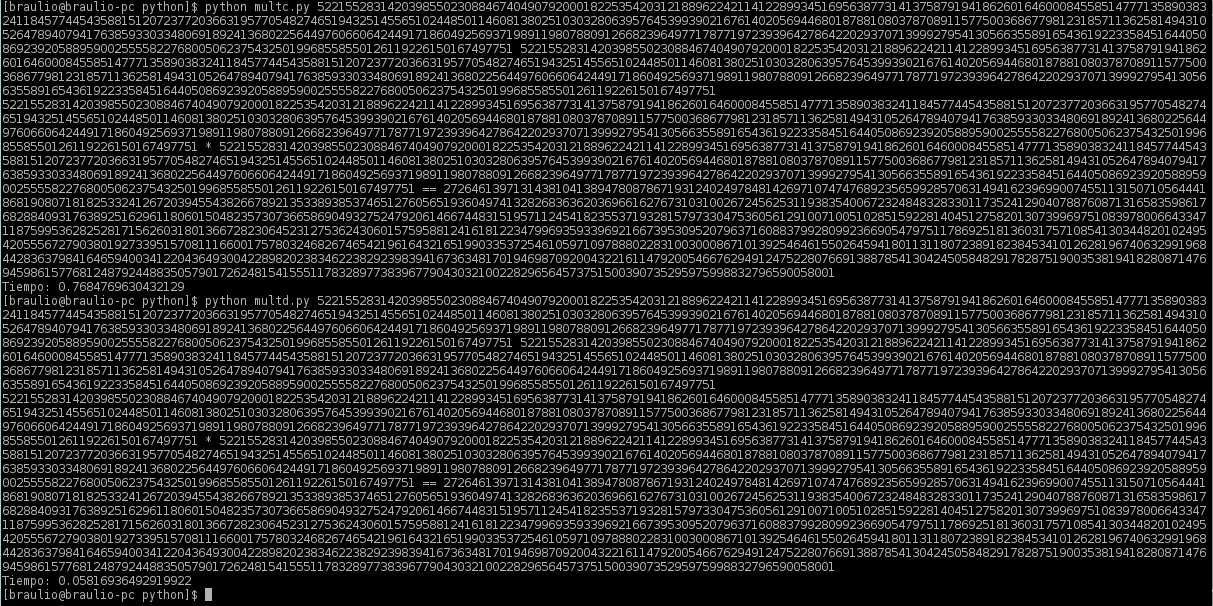
\includegraphics[width=0.8\textwidth]{figura1}
\caption{Alg. clasico = $0.7684769630432129$s. vs. Algoritmo DyV = $0.05816936492919922$s.}
\label{comparativa}
\end{figure}
\end{center}

El algoritmo tiene una orden de eficiencia que viene definido por la siguiente ecuación:
\begin{displaymath}
  t(n) = 3 \cdot t\left(\frac{n}{2}\right)+d'\cdot n
\end{displaymath}

Esta ecuación surge de las tres llamadas recursivas al procedimiento mas la combinación de los resultados. La ecuación del algoritmo pertenece a $O(n^{\log_23}) \approx O(n^{1.59}$. Asintóticamente el algoritmo es mejor, pero para tamaños pequeños, la división en subproblemas y la combinación de los resultados parciales supone que solo haya una mejora para enteros mayores de 500 bits. La \hyperref[figura2]{Figura \ref*{figura2}} es un ejemplo de ello:

\begin{center}
\begin{figure}[!h]
\centering
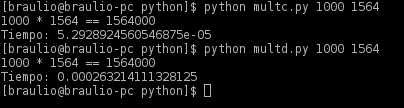
\includegraphics[width=0.44\textwidth]{figura2}
\caption{Alg. clasico = $5.2928924560546875e-05$s. vs. Algoritmo DyV = $0.000263214111328125$s.}
\label{figura2}
\end{figure}
\end{center}

\mypython[label="Karatsuba\&Ofman"]{../Multiplicacion_Enteros_Largos/multd.py}

Como conclusión, el algoritmo solo es rentable para aquellos enteros que son de un tamaño, en la práctica, mayores de $500bits$.
//
Esta práctica, junto con la de \hyperref[bb]{Branch\&Bound} la he hecho con Marta Gómez Macías por falta de tiempo.

\chapter{\textcolor[rgb]{0.1,0.2,1}Práctica 4: \textcolor[rgb]{0.1,0.2,1}Algoritmos \textcolor[rgb]{0.1,0.2,1}Greedy}

\section{\textcolor[rgb]{0.1,0.2,1}Enunciado}

Implementar el problema de la \textbf{\textcolor[rgb]{0.1,0.2,1}{mochila fraccional}} utilizando un \textit{\textcolor[rgb]{0.1,0.2,1}{algoritmo greedy}}.

\subsection{\textcolor[rgb]{0.1,0.2,1}Solución}

Para este problema he propuesto una estructura llamada \verb|objeto| que contiene el \verb|beneficio| y el \verb|peso| de un objeto, donde ambos pueden ser valores reales; y una estructura llamada \verb|Opcion| que recoge el \verb|objeto| y un campo \verb|porcentaje|. Este campo es la proporción del objeto que tomamos.

El algoritmo se basa en de una lista ordenada de \verb|objeto| por beneficio por unidad de peso, escogemos el último ya que la \verb|STL| ordena los elementos de menor a mayor, y lo vamos metiendo en la mochila mientras quede espacio y objetos para meter. Este objeto pasará a ser el que hay en \verb|Opcion.o| y \verb|O.porcentaje = 1|  Una vez que el peso total mas el del objeto que hemos cogido supera el peso de la mochila (y aún queda espacio en la mochila), fraccionamos el objeto con la siguiente razón:
\begin{displaymath}
  porcentaje = \frac{PesoMochila - PesoActual}{PesoDelObjeto}
\end{displaymath}

Esto nos da la proporción del objeto que se mete en la mochila. Tras esto, se iguala el peso actual al peso de la mochila y se sale de la función.
\newpage
\mycpp[label="MochilaFraccional"]{../Mochila_Greedy/src/Greedy.cpp}

\newpage

A continuación, se muestran dos ejemplos de ejecución para la mochila fraccional para dos ejemplos:

\begin{enumerate}[$\blacksquare$]
  \item El primer ejemplo de ejecución tiene los siguientes datos:
  \begin{enumerate}[$\spadesuit$]
    \item Objetos\footnote{El primer número del objeto indica el beneficio, mientras que el segundo indica el peso de dicho objeto.}: [55, 2], [1,2]
    \item Peso de la mochila: 2.5
  \end{enumerate}
  \item El segundo ejemplo de ejecución tiene:
  \begin{enumerate}[$\spadesuit$]
    \item Objetos: [7, 2], [4, 3], [2, 4], [3, 6]
    \item Peso de la mochila: 11
  \end{enumerate}
\end{enumerate}

\begin{center}
\begin{figure}[!h]
\centering
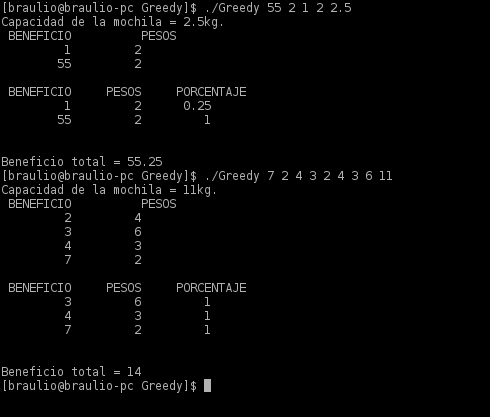
\includegraphics[width=0.5\textwidth]{figura3}
\caption{Ejemplos de ejecución}
\label{figura3}
\end{figure}
\end{center}

\chapter{\textcolor[rgb]{0.1,0.2,1}Práctica 5: Programación Dinámica}

\section{\textcolor[rgb]{0.1,0.2,1}Enunciado}

Implementar el problema de la \textbf{\textcolor[rgb]{0.1,0.2,1}{mochila 0/1}} utilizando \textit{\textcolor[rgb]{0.1,0.2,1}{programación dinámica}}.

\subsection{\textcolor[rgb]{0.1,0.2,1}Solución}

Siguiendo la definición del problema de la mochila con la versión para programación dinámica, tenemos los siguientes casos:

\begin{description}
  \item [Si no se coge el objeto $k$]: Nuestra función mochila será la misma pero analizaremoos los $k-1$ objetos restantes.
  $$Mochila(k,m) = Mochila(k-1,m)$$.
  \item [Si se coge:] Nuestra función mochila nos devuelve el beneficio del objeto $k$ mas el beneficio de los $k-1$ objetos restantes.
  $$Mochila(k,m) = b_k + Mochila(k-1, m-p_k)$$
  \item [Valor çoptimo:] El que dé el mayor beneficio:
  $$Mochila(k,mo) = max\{Mochila(k-1,m), b_k + Mochila(k-1, m-p_k)\}$$
\end{description}

Y los siguientes casos base:

\begin{enumerate}[---]
  \item Si $m=0$, no se pueden incluir objetos:
  $$Mochila(k,0) = 0$$
  \item Si $k=0$, tampoco se pueden incluir:
  $$Mochila(k,0) = 0$$
  \item Y si $m$ o $k$ son negativos, tenemos:
  $$Mochila(k<0,m<0) = -\infty$$
  Esto es solo para que cuando uno de los dos sea negativo, directamente se coja la otra opción directamente y no haya problemas en los accesos a memoria en los arrays que conforman la tabla.
\end{enumerate}

Todo esto conforma esta ecuación:

\begin{equation*}
Mochila(k,m)= 
\begin{cases}
0 & \textit{si } k = 0 \textit{ ó } m=0, \\
-\infty & \textit{si } k < 0 \textit{ ó } m < 0, \\
max\{Mochila(k-1,m), b_k + Mochila(k-1, m-p_k)\} &
\end{cases}
\end{equation*}

Siguiendo con esto, rellenamos los casos base de la tabla, que es la fila y columna 0 con 0, y seguimos rellenando la tabla siguiendo la fórmula.

Para recomponer la solución, se utiliza un algoritmo muy sencillo que va recorriendo la tabla desde el final hasta el principio, donde si el elemento que está una fila más arriba del actual es distinto, quiere decir que el objeto se ha cogido y retrocedemos una columna. En caso contrario, seguimos retrocediendo por las filas.

\mycpp[label="Mochila0/1"]{../Mochila_Programacion_Dinamica/src/mochila_bp.cpp}

La ejecución del programa da los siguientes resultados:

\begin{center}
\begin{figure}[!h]
\centering
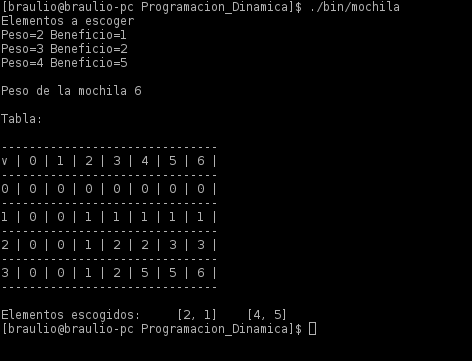
\includegraphics[width=0.8\textwidth]{figura4}
\caption{Ejemplo de ejecución}
\label{figura4}
\end{figure}
\end{center}

\chapter{\textcolor[rgb]{0.1,0.2,1}Práctica 6: Branch\&Bound}
\label{bb}

\section{\textcolor[rgb]{0.1,0.2,1}Enunciado}

Implementar el algoritmo de la mochila 0/1 usando un algoritmo \textbf{\textit{\textcolor[rgb]{0.1,0.2,1}}{Branch\&Bound}}.

\subsection{\textcolor[rgb]{0.1,0.2,1}Solución}

Para resolver el ejercicio se ha planteado un árbol binario que coge los elementos del conjunto inicial en un \verb|multiset<Elemento>| ya que inserta los elementos de forma ordenada en función de la proporción de beneficio por unidad de peso y como por debajo tiene un \verb|rb_tree|, el moverse por el conjunto es muy rápido. 

El algoritmo irá cogiendo el último elemento del conjunto (porque la \verb|STL| ordena los elementos de menor a mayor) ya que es el mejor de los objetos posibles e irá generando un árbol binario, analizando primero el coger el objeto y más tarde el de no cogerlo.

Las cotas que se usarán para ramificar y podar son:
\begin{description}
  \item [CI:] Valor actual que llevamos acumulado.
  \item [BE:] Beneficio estimado que calcularemos con un algoritmo Greedy. Este algoritmo greedy recoge el beneficio acumulado que llevemos, mas el beneficio que obtiene cogiendo los mejores objetos que puedan entrar en la mochila, sin pararse a mirar si es conveniente o no.
  \item [CS:] Beneficio que se obtiene sumando el beneficio actual y el beneficio que obtiene el algoritmo greedy en su versión fraccional.
\end{description}

Los nodos pasarán a analizarse si la cota superior es mayor que nuestra cota $C$,que es el valor actual que tenemos. Si es un nodo hoja y su valor es mayor que la cota, se coge el nodo y la tupla asociada. Si aún no es un nodo hoja, se mete en la lista de nodos vivos ($LNV$) para procesarlo más tarde.

El árbol que desarrolla el algorítmo es algo similar a este:

\begin{center}
\begin{figure}[!h]
\centering
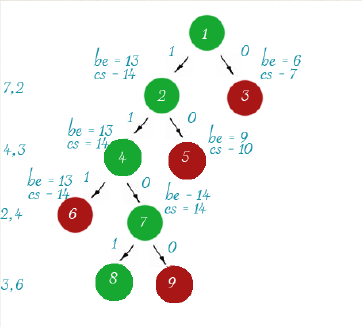
\includegraphics[width=0.6\textwidth]{figura5}
\caption{Árbol binario desarrollado}
\label{figura5}
\end{figure}
\end{center}

\mycpp[label="MochilaBB"]{../Mochila_Branch_and_Bound/src/mochila_branch_bound.cpp}

Un ejemplo de ejecución es el siguiente:

\begin{center}
\begin{figure}[!h]
\centering
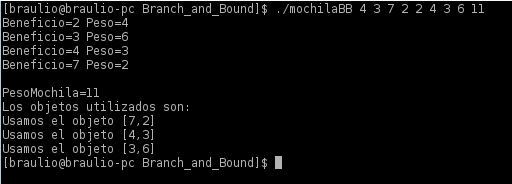
\includegraphics[width=0.8\textwidth]{figura6}
\caption{Ejemplo de ejecución}
\label{figura6}
\end{figure}
\end{center}

\end{document}